% "Станет проще"

\documentclass[a4paper,12pt]{article} % тип документа

% report, book

%  Русский язык

\usepackage[T2A]{fontenc}			% кодировка
\usepackage[utf8]{inputenc}			% кодировка исходного текста
\usepackage{graphicx}
\usepackage[english,russian]{babel}	% локализация и переносы


%отступ
\usepackage[left=3cm,right=3cm,
    top=3cm,bottom=3cm,bindingoffset=0cm]{geometry}

% Математика
\usepackage{amsmath,amsfonts,amssymb,amsthm,mathtools} 
\usepackage{csvsimple}
\usepackage{multirow}


\usepackage{wasysym}
\usepackage{subcaption}
\usepackage{verbatim}
\usepackage{hyperref}
\usepackage{float}
\usepackage{enumerate}
%Заговолок
\graphicspath{ {images/} }


\begin{titlepage}
\author{Соловьянов Михаил }
\title{Задание 1. Электродинамика.  Цепи постоянного тока}
\date{\today}
\end{titlepage}



\begin{document} % начало документа
\maketitle

\begin{figure}[H]
\centering
  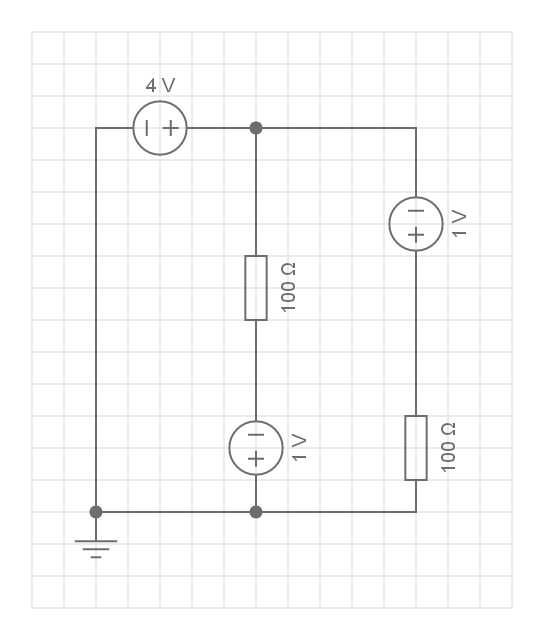
\includegraphics[width=0.5\linewidth]{circuit1.png}
  \caption{К задаче 1.}
  \label{fig1}
\end{figure}



\begin{figure}[H]
\centering
  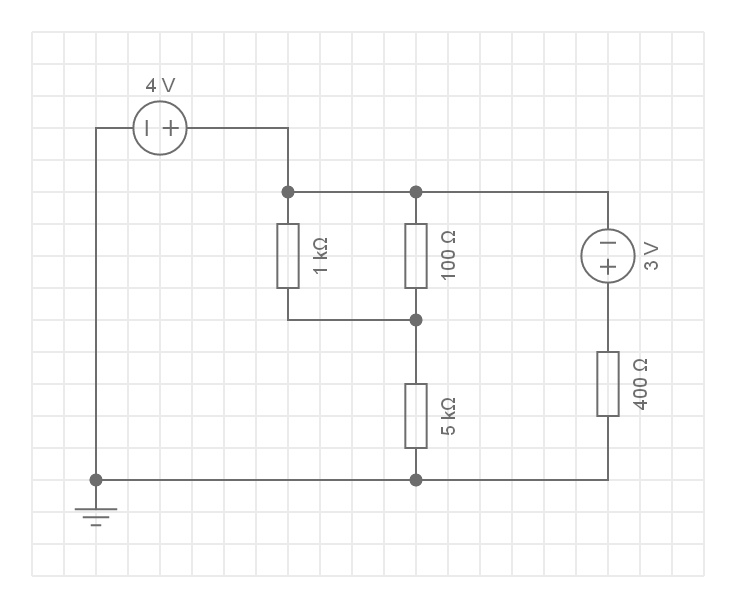
\includegraphics[width=0.5\linewidth]{circuit2.png}
  \caption{К задаче 2.}
  \label{fig2}
\end{figure}


\begin{figure}[H]
\centering
  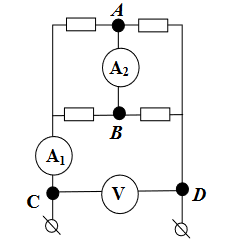
\includegraphics[width=0.5\linewidth]{3.png}
  \caption{К задаче 3.}
  \label{fig3}
\end{figure}

\begin{figure}[H]
\centering
  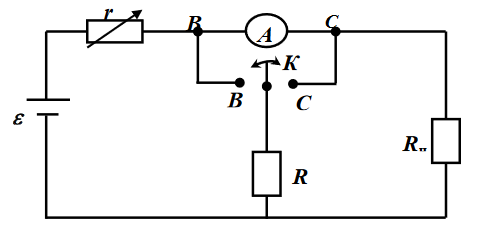
\includegraphics[width=0.5\linewidth]{4.png}
  \caption{К задаче 4.}
  \label{fig4}
\end{figure}

\section{Контрольные вопросы}
\begin{enumerate}

\item Сформулировать первый и второй законы Кирхгофа.
\item Имеется источник напряжения, я подключаю к нему два разных резистора по очереди. Измениться ли напряжение на истонике напряжения? А ток? Источник идеальный.
\end{enumerate}


\section{Задачи}
\begin{enumerate}
\item Рассчитать токи в цепи (рис. \ref{fig1} )
\item Рассчитать токи в цепи  (рис. \ref{fig2} )

\item В  цепи,которая  изображена  на рисунке, амперметр $A_2$ показывает  силу тока 2А.  Найдите  показания  амперметра $A_1$,  если  известно,  что  резисторы  имеют сопротивления 1Ом,2Ом,3Ом, и 4Ом, а вольтметр V показывает напряжение 10В. Все приборы считать идеальными. (3.26[1])  (рис. \ref{fig3} )

\item В нейтральном  положении  ключа Ксила  тока  в  цепи  равна 0,1А. При подключении к контакту Вамперметр показывает силу тока 0,05А. При подключении к  контакту Самперметр показывает  0,3А.  Найти отношение    мощности нагревателя $R_n $ к   полной потребляемой  мощности цепи,  т.е.  кпд  во  всех случаях.  Источник  и  амперметр  считать  идеаль-ными. Сопротивление нагревателя $R_n $ постоянно во всех случаях  (рис. \ref{fig4} ) 3.20[1]

\end{enumerate}





\end{document}